\documentclass[12pt]{article}
\usepackage{homework}
\pagestyle{fancy}

% assignment information
\def\course{Electromagnetism}
\def\assignmentno{Problem Sheet 2}
\def\assignmentname{Electric and Magnetic Fields in Matter}
\def\name{Xin, Wenkang}
\def\time{\today}

\begin{document}

\begin{titlepage}
    \begin{center}
        \large
        \textbf{\course}

        \vfill

        \Huge
        \textbf{\assignmentno}

        \vspace{1.5cm}

        \large{\assignmentname}

        \vfill

        \large
        \name

        \time
    \end{center}
\end{titlepage}


%==========
\pagebreak
\section*{Electric Field in Matter}
%==========


\problem{2.1}{Capacitance and dielectrics}

\subproblem{a}
Using a small box-shape Gaussian surface, the field produced by a large plate carrying a uniform surface charge density $\sigma$ is $\sigma/2\epsilon_{0}$ as computed via Gauss' law. The parallel plate capacitor has two such plates, so the field between the plates is a superposition of the fields produced by each plate:

\begin{equation}
    E_{0} = \frac{Q_{0}/A}{2\epsilon_{0}} - \left( \frac{-Q_{0}/A}{2\epsilon_{0}} \right) = \frac{Q_{0}}{A\epsilon_{0}}
\end{equation}

As the field is uniform, the potential difference between the plates is simply $V_{0} = E_{0}d = Q_{0}d/A\epsilon_{0}$. The capacitance is then $C = Q_{0}/V_{0} = A\epsilon_{0}/d$.

The potential energy stored in the capacitor can be computed by integrating the energy density over the volume between the plates:

\begin{equation}
    U_{0} = \frac{\epsilon_{0}}{2} \int_{V} E_{0}^{2} \, \mathrm{d}V = \frac{\epsilon_{0}}{2} \frac{Q_{0}^{2}}{A^{2}\epsilon_{0}^{2}} \int_{V} \, \mathrm{d}V = \frac{Q_{0}^{2}d}{2A\epsilon_{0}}
\end{equation}

\subproblem{b}
Consider the relationship between the potential difference and the charge on the capacitor:

\begin{equation}
    V = \frac{Qd}{\epsilon_{0}A}
\end{equation}

The dielectric material inserted causes a change in the permittivity $\epsilon_{0} \to \epsilon_{r} \epsilon_{0} > \epsilon_{0}$. Given constant $V$, the charge on the capacitor is then $Q \to \epsilon_{r}Q > Q$.

Apply Gauss' law for electric displacement $\mathbf{D}$ with a small box-shape Gaussian surface:

\begin{equation}
    \begin{split}
        \oint_{S} \mathbf{D} \cdot \mathrm{d}\mathbf{S} &= Q_{f} \\
        D \alpha &= \frac{Q\alpha}{A} \\
        \epsilon_{0} E + P &= \frac{Q}{A}
    \end{split}
\end{equation}

which gives $E = (Q/A - P)/\epsilon_{0}$.

Assuming a linear dielectric with the polarization $P = \epsilon_{0} \chi_{e} E$, the electric field is then:

\begin{equation}
    E = \frac{Q}{A\epsilon_{0}(1 + \chi_{e})}
\end{equation}

Since the potential is kept constant, the field is also constant so that $E = E_{0}$, which gives the relation:

\begin{equation}
    \frac{Q}{A\epsilon_{0}(1 + \chi_{e})} = \frac{Q_{0}}{A\epsilon_{0}}
\end{equation}

or $Q = (1 + \chi_{e}) Q_{0}$ as expected.

The capacitance is then $C = Q/V_{0} = (1 + \chi_{e})C_{0}$, and the change in the potential energy is:

\begin{equation}
    \Delta U = \frac{Q^{2}d}{2A\epsilon_{r}\epsilon_{0}} - \frac{Q_{0}^{2}d}{2A\epsilon_{0}} = \chi_{e} U_{0}
\end{equation}

\subproblem{c}
Still consider the previous relationship but keep the charge constant. The increase in permittivity causes a decrease in the potential difference $V \to V/\epsilon_{r} < V$.

The capacitance is a property of geometry and material (permittivity) so it is unchanged, i.e., $C = (1 + \chi_{e})C_{0}$. The change in the potential energy is:

\begin{equation}
    \Delta U = \frac{Q_{0}^{2}d}{2A\epsilon_{r}\epsilon_{0}} - \frac{Q_{0}^{2}d}{2A\epsilon_{0}} = -\frac{\chi_{e}}{1 + \chi_{e}} U_{0}
\end{equation}
\qed


\problem{2.2}{Capacitor half-filled with a dielectric}

\subproblem{a}
Label the regions from $1$ to $4$ from left to right as depicted in the figure. Apparently the electric fields and polarisations in region $1$ and $4$ are zero. Applying Gauss' law in region $2$ and $3$ gives:

\begin{equation}
    \begin{split}
        D_{2} \alpha &= \sigma \alpha = (\epsilon_{0} E_{2} + P) \alpha \\
        D_{3} \alpha &= \sigma \alpha = \epsilon_{0} E_{3} \alpha
    \end{split}
\end{equation}

Solving the equations gives $E_{2} = \sigma/\epsilon_{0} \epsilon_{r}$, $P = (1 - 1/\epsilon_{r}) \sigma$, and $E_{3} = \sigma/\epsilon_{0}$. Thus:

\begin{equation}
    \begin{split}
        \mathbf{D}_{2} &= \mathbf{D}_{3} = \sigma \hat{x} \\
        \mathbf{E}_{2} &= \frac{\sigma}{\epsilon_{0} \epsilon_{r}} \hat{x} \\
        \mathbf{E}_{3} &= \frac{\sigma}{\epsilon_{0}} \hat{x} \\
        \mathbf{P} &= \left( 1 - \frac{1}{\epsilon_{r}} \right) \sigma \hat{x}
    \end{split}
\end{equation}

where $\hat{x}$ is the unit vector pointing from the positive plate to the negative one.

\subproblem{b}
Taking the negative plate as the reference point, the potential difference between the plates is:

\begin{equation}
    \begin{split}
        V &= \int_{0}^{d} E_{2} \, \mathrm{d}x + \int_{d}^{2d} E_{3} \, \mathrm{d}x \\
        &= \left( \frac{1}{\epsilon_{0} \epsilon_{r}} + \frac{1}{\epsilon_{0}} \right) \sigma d \\
    \end{split}
\end{equation}

The capacitance is:

\begin{equation}
    C = \frac{\sigma A}{V} = \frac{A/d}{1/\epsilon_{0} \epsilon_{r} + 1/\epsilon_{0}}
\end{equation}

Note that:

\begin{equation}
    \frac{1}{C} = \frac{d}{A} \left( \frac{1}{\epsilon_{0} \epsilon_{r}} + \frac{1}{\epsilon_{0}} \right) = \frac{1}{C_{1}} + \frac{1}{C_{2}}
\end{equation}

where $C_{1}$ is the capacitance of the left half and $C_{2}$ is the capacitance of the right half.

This is as though the capacitance of two capacitors in series.

\subproblem{c}
As the polarisation is constant, there is no volume bound density since $\nabla \cdot \mathbf{P} = 0$. On the interface between region $1$ and $2$:

\begin{equation}
    \sigma_{b} = -p = -\left( 1 - \frac{1}{\epsilon_{r}} \right) \sigma
\end{equation}

On the interface between region $2$ and $3$:

\begin{equation}
    \sigma_{b} = p = \left( 1 - \frac{1}{\epsilon_{r}} \right) \sigma
\end{equation}

Using all surface charge densities, the electric field in four regions are:

\begin{equation}
    \begin{split}
        \mathbf{E}_{1} &= \frac{\sigma}{2\epsilon_{0}} \left[ -\frac{1}{\epsilon_{r}} - \left( 1 - \frac{1}{\epsilon_{r}} \right) + 1 \right] \hat{x} = 0 \\
        \mathbf{E}_{2} &= \frac{\sigma}{2\epsilon_{0}} \left[ \frac{1}{\epsilon_{r}} - \left( 1 - \frac{1}{\epsilon_{r}} \right) + 1 \right] \hat{x} = \frac{\sigma}{\epsilon_{0}\epsilon_{r}} \hat{x} \\
        \mathbf{E}_{3} &= \frac{\sigma}{2\epsilon_{0}} \left[ \frac{1}{\epsilon_{r}} + \left( 1 - \frac{1}{\epsilon_{r}} \right) + 1 \right] \hat{x} = \frac{\sigma}{\epsilon_{0}} \hat{x} \\
        \mathbf{E}_{4} &= \frac{\sigma}{2\epsilon_{0}} \left[ \frac{1}{\epsilon_{r}} + \left( 1 - \frac{1}{\epsilon_{r}} \right) - 1 \right] \hat{x} = 0
    \end{split}
\end{equation}

which are the same as the results in part (a).
\qed


\problem{2.3}{Force on a dielectric}

\subproblem{a}
By Gauss' law for electric displacement $\mathbf{D}$, the electric field in the dielectric is:

\begin{equation}
    E' = \frac{\sigma'}{\epsilon_{0} \epsilon_{r}}
\end{equation}

whereas in the electric field in vacuum region is:

\begin{equation}
    E'' = \frac{\sigma''}{\epsilon_{0}}
\end{equation}

As $\mathbf{E}_{\parallel}$ is continuous across a boundary, we must have $E' = E''$ or that $\sigma' = \epsilon_{r} \sigma''$. The total charge on the upper plate is given by:

\begin{equation}
    Q = w \left[ \sigma' x + \sigma''(L - x) \right]
\end{equation}

which means that $\sigma''$ can be expressed as:

\begin{equation}
    \sigma'' = \frac{1}{L + (\epsilon_{r} - 1)x} \frac{Q}{w} = \frac{Q}{sw}
\end{equation}

where we have defined $s \equiv L + (\epsilon_{r} - 1)x$.

The potential difference between the plates is just $V = E'' d$ and the potential energy stored in the capacitor consists of two parts:

\begin{equation}
    \begin{split}
        U &= \frac{\epsilon_{0}}{2} E''^{2} (L-x)wd + \frac{\epsilon_{0} \epsilon_{r}}{2} E'^{2} xwd \\
        &= \frac{\epsilon_{0}wd}{2} \left( \frac{\sigma''}{\epsilon_{0}} \right)^{2} (L - x + \epsilon_{r} x) \\
        &= \frac{wd}{2\epsilon_{0}} \left( \frac{Q}{sw} \right)^{2} s \\
        &= \frac{Q^{2}d}{2w} \frac{1}{L + (\epsilon_{r} - 1)x}
    \end{split}
\end{equation}

Differentiating the energy with respect to $x$ gives:

\begin{equation}
    \mathrm{d}U = -\frac{Q^{2}d}{2w} \frac{\epsilon_{r} - 1}{[L + (\epsilon_{r} - 1)x]^{2}} \, \mathrm{d}x
\end{equation}

so that

\begin{equation}
    F = -\frac{\mathrm{d}U}{\mathrm{d}x} = \frac{Q^{2}d}{2w} \frac{\epsilon_{r} - 1}{[L + (\epsilon_{r} - 1)x]^{2}} > 0
\end{equation}

This means that the force tends to push the dielectric into the capacitor.

\subproblem{b}
If $V = E'' d$ is kept constant, we have $E''$ constant so that $\sigma''$ is constant. The potential energy is:

\begin{equation}
    U = \frac{wd\sigma''^{2}}{2\epsilon_{0}} \left[ L + (\epsilon_{r} - 1)x \right]
\end{equation}

and the force is:

\begin{equation}
    \begin{split}
        F &= -\frac{wd\sigma''^{2}}{2\epsilon_{0}} (\epsilon_{r} - 1) \\
        &= -\frac{wd}{2\epsilon_{0}} \left( \frac{Q}{sw} \right)^{2} (\epsilon_{r} - 1) \\
        &= -\frac{Q^{2}d}{2w} \frac{\epsilon_{r} - 1}{[L + (\epsilon_{r} - 1)x]^{2}} < 0
    \end{split}
\end{equation}

which has the same magnitude as the previous result but with opposite direction.

\subproblem{c}
No, the force experienced by the dielectric depends on the existence of the fringe field. In fact, it is not correct to assume zero field outside the capacitor as $\mathbf{E}_{\parallel}$ would not be continuous across the boundary. In this model, the information on the force is contained in the potential energy so that we can compute the force by differentiating it with respect to $x$.
\qed


\problem{2.4}{Sphere with a frozen-in polarization}

\subproblem{a}
Given $\mathbf{P} = k \mathbf{r}$, the surface charge density on the sphere is:

\begin{equation}
    \sigma_{b} = \mathbf{P} \cdot \hat{r} = kR
\end{equation}

where $\mathbf{P}$ is evaluated at the surface of the sphere.

The volume bound charge density is:

\begin{equation}
    \rho_{b} = -\nabla \cdot \mathbf{P} = -3k
\end{equation}

\subproblem{b}
Inside the sphere, only volume charge density contribute to Gauss' law for electric field:

\begin{equation}
    E (4\pi r^{2}) = \frac{1}{\epsilon_{0}} \left( -3k \frac{4}{3} \pi r^{3} \right)
\end{equation}

or:

\begin{equation}
    \mathbf{E} = -\frac{kr}{\epsilon_{0}} \hat{r}
\end{equation}

Outside the sphere, both surface and volume charge densities contribute to Gauss' law:

\begin{equation}
    E (4\pi r^{2}) = \frac{1}{\epsilon_{0}} \left[ kR (4\pi R^{2}) - 3k \frac{4}{3} \pi R^{3} \right] = 0
\end{equation}

Thus, the electric field is given by:

\begin{equation}
    \mathbf{E} =
    \begin{cases}
        -k \mathbf{r}/\epsilon_{0} & r < R \\
        0                          & r > R
    \end{cases}
\end{equation}

\subproblem{c}
Inside the sphere, the electric displacement is $\mathbf{D} = \epsilon_{0} \mathbf{E} + \mathbf{P} = \mathbf{0}$. Outside the sphere, the electric displacement is still zero as there is no electric field or polarisation. Thus, the electric displacement is zero everywhere. This is expected as there is no free charge in the system. The dielectric is not linear as $\mathbf{P}$ is not proportional to $\mathbf{D}$.
\qed


%==========
\pagebreak
\section*{Magnetic Field in Matter}
%==========


\problem{2.5}{$\mathbf{B}$, $\mathbf{H}$, and $\mathbf{M}$ in a bar magnet}

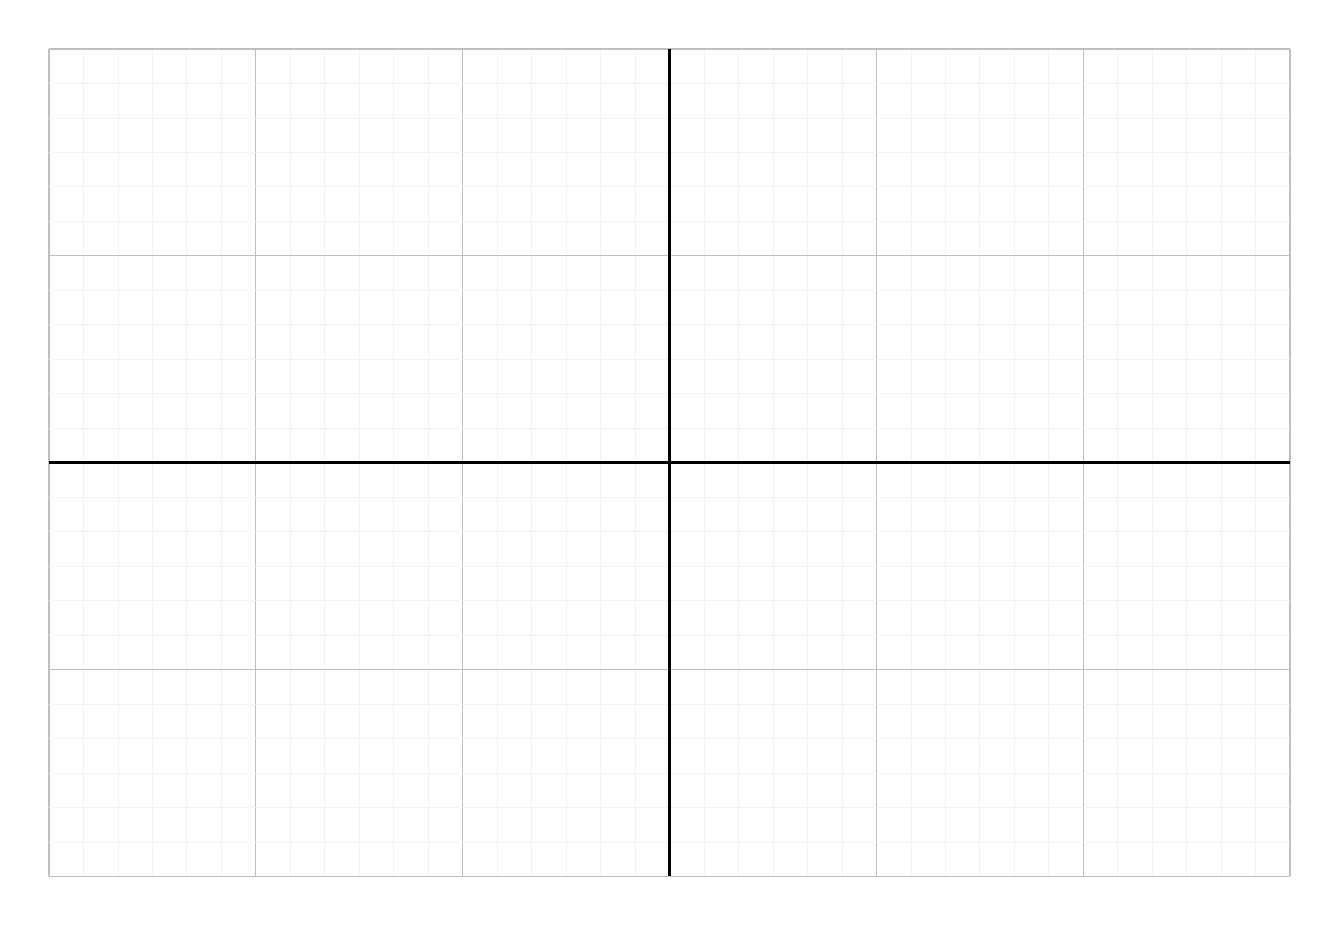
\begin{tikzpicture}[scale = 2.3]
    \begin{axis}[
            title = ,
            xmin=-15, xmax=15,
            ymin=-10, ymax=10,
            grid=both,
            grid style={line width=.1pt, draw=gray!10},
            major grid style={line width=.2pt,draw=gray!50},
            axis lines*=middle,
            minor tick num=5,
            xtick style={draw=none},ytick style={draw=none},
            xticklabels={, ,},yticklabels={, ,},
            axis equal image
        ]
    \end{axis}
\end{tikzpicture}

\qed


\problem{2.6}{Cylinder with a frozen-in magnetization}

\subproblem{a}
Given $\mathbf{M} = kr \hat{z}$, the surface bound current density on the cylinder is:

\begin{equation}
    \mathbf{K}_{b} = \mathbf{M} \times \hat{z} = kR \hat{\phi}
\end{equation}

where $\mathbf{M}$ is evaluated at the surface of the cylinder.

The volume bound current density is:

\begin{equation}
    \mathbf{J}_{b} = \nabla \times \mathbf{M} = -k \hat{\phi}
\end{equation}

Since both $\mathbf{K}_{b}$ and $\mathbf{J}_{b}$ are circumferential, we expect the magnetic field to be along the axis of the cylinder. Due to azimuthal symmetry and infinite length, it can be asserted that the field has no $z$ or $\phi$ dependence.

Consider a point $(h, 0, 0)$ on the perpendicular bisector of the cylinder. Using Biot-Savart law, we first compute the magnetic field due to the surface bound current density:

\begin{equation}
    \begin{split}
        \mathbf{B}_{1} &= \frac{\mu_{0}}{4\pi} \int_{S} \frac{\mathbf{K}_{b} \times \mathbf{r}'}{r'^{3}} \, \mathrm{d}S \\
        &= -\frac{\mu_{0}kR^{2}}{4\pi} \int_{-\infty}^{\infty} \int_{0}^{\phi} \frac{\hat{\phi} \times [z \hat{z} + (R-h) \hat{r}]}{[z^{2} + (R-h)^{2}]^{3/2}} \, \mathrm{d}\phi \, \mathrm{d}z \\
        &= -\frac{\mu_{0}kR^{2}}{2} \int_{-\infty}^{\infty} \frac{\hat{\phi} \times [z \hat{z} + (R-h) \hat{r}]}{[z^{2} + (R-h)^{2}]^{3/2}} \, \mathrm{d}z \\
    \end{split}
\end{equation}

where $\mathbf{r}' = -z \hat{z} - (R-h) \hat{r}$ is the vector from the area element to the point of interest and $\mathrm{d}S = R \, \mathrm{d}\phi \, \mathrm{d}z$ is the area element.

Any $\phi$ component in $\mathbf{r}'$ can be ignored as it gives zero contribution to the integral. The first part of the integrand is along the $r$ direction so it can be discarded. The second part is along the negative $z$ direction and evaluates to $-2/(h-R)$, so that:

\begin{equation}
    \mathbf{B}_{1} = \mu_{0}k \frac{R^{2}}{R-h} \hat{z}
\end{equation}

The magnetic field due to the volume bound current density is:

\begin{equation}
    \begin{split}
        \mathbf{B}_{2} &= \frac{\mu_{0}}{4\pi} \int_{V} \frac{\mathbf{J}_{b} \times \mathbf{r}'}{r'^{3}} \, \mathrm{d}V \\
        &= \frac{\mu_{0}k}{4\pi} \int_{-\infty}^{\infty} \int_{0}^{\phi} \int_{0}^{R} \frac{\hat{\phi} \times [z \hat{z} + (r-h) \hat{r}]}{[z^{2} + (r-h)^{2}]^{3/2}} r \, \mathrm{d}r \, \mathrm{d}\phi \, \mathrm{d}z \\
        &= \frac{\mu_{0}k}{2} \int_{-\infty}^{\infty} \int_{0}^{R} \frac{\hat{\phi} \times [z \hat{z} + (r-h) \hat{r}]}{[z^{2} + (r-h)^{2}]^{3/2}} r \, \mathrm{d}r \, \mathrm{d}z \\
    \end{split}
\end{equation}

where $\mathbf{r}'$ is defined similarly as before and $\mathrm{d}V = r \, \mathrm{d}r \, \mathrm{d}\phi \, \mathrm{d}z$ is the volume element.

The first part of the integrand can be similarly ignored and the second part requires us to change to polar coordinates. Consider the change of variables:

\begin{equation}
    \begin{split}
        r' &= r - h = \rho \cos{\theta} \\
        z &= \rho \sin{\theta}
    \end{split}
\end{equation}

The integral becomes:

\begin{equation}
    \begin{split}
        &\int_{-\infty}^{\infty} \int_{-h}^{R-h} \frac{r'(r'+h)}{(z^{2} + r'^{2})^{3/2}} \, \mathrm{d}r' \, \mathrm{d}z \\
        = &\int_{0}^{\pi} \int_{0}^{\frac{R-h}{\sin{\theta}}} \left( \frac{\cos^{2}{\theta}}{\rho} + \frac{h}{\rho^{2}} \cos{\theta} \right) \rho \, \mathrm{d}\rho \, \mathrm{d}\theta + \int_{\pi}^{2\pi} \int_{0}^{-\frac{h}{\sin{\theta}}} \left( \frac{\cos^{2}{\theta}}{\rho} - \frac{h}{\rho^{2}} \cos{\theta} \right) \rho \, \mathrm{d}\rho \, \mathrm{d}\theta \\
        = &\int_{0}^{\pi} \left[ \frac{(R-h)^{2}}{2} \cot{\theta} + h(R - h) \cot{\theta} \right] \, \mathrm{d}\theta + \int_{\pi}^{2\pi} \left( \frac{h^{2}}{2} \cot{\theta} + h^{2} \cot{\theta} \right) \, \mathrm{d}\theta \\
        = &\frac{(R-h)^{2}}{2} \left[ \theta + \cot{\theta} \right]_{0}^{\pi} + h(R - h) \left[ \ln{\sin{\theta}} \right]_{0}^{\pi} + \frac{h^{2}}{2} \left[ \theta + \cot{\theta} \right]_{\pi}^{2\pi} + h^{2} \left[ \ln{\sin{\theta}} \right]_{\pi}^{2\pi} \\
        = &2\left( R + h \ln{\frac{\left\lvert R-h \right\rvert}{h}} \right)
    \end{split}
\end{equation}

Returning to the magnetic field:

\begin{equation}
    \mathbf{B}_{2} = -\mu_{0}k \left( R + h \ln{\frac{\left\lvert R-h \right\rvert}{h}} \right) \hat{z}
\end{equation}

Combining the two parts, we obtain the full expression for the magnetic field:

\begin{equation}
    \mathbf{B}(h) = \mu_{0}k \left[ \frac{R^{2}}{R-h} - \left( R + h \ln{\frac{\left\lvert R-h \right\rvert}{h}} \right) \right] \hat{z}
\end{equation}

which becomes $0$ as $h \to 0$.

\subproblem{b}
Since there is no free current in the system, $\mathbf{H} = \mathbf{0}$ everywhere. Outside the cylinder, there is no magnetisation so that $\mathbf{B} = \mu_{0} \mathbf{H} = \mathbf{0}$. Inside the cylinder:

\begin{equation}
    \mathbf{H} = \frac{\mathbf{B}}{\mu_{0}} - kr \hat{z} = \mathbf{0}
\end{equation}

so that $\mathbf{B} = \mu_{0} kr \hat{z}$.
\qed


\problem{2.7}{Magnetic field in a coaxial cable}
Ampere's law for the auxiliary field $\mathbf{H}$ gives:

\begin{equation}
    \oint \mathbf{H} \cdot \mathrm{d}\mathbf{l} = H 2\pi r = -I
\end{equation}

where we take the positive direction of the current to be $z$ direction.

This gives $\mathbf{H} = -I/(2\pi r) \hat{\phi}$ so that:

\begin{equation}
    \mathbf{B} = \mu_{0} \mu_{r} \mathbf{H} = -\frac{\mu_{0} (1 + \chi_{m}) I}{2\pi r} \hat{\phi}
\end{equation}

Given the auxiliary field, the magnetisation is just $\mathbf{M} = \chi_{m} \mathbf{H} = -\chi_{m} I/(2\pi r) \hat{\phi}$. This gives the bound current densities:

\begin{equation}
    \begin{split}
        \mathbf{J}_{b} &= \nabla \times \mathbf{M} = 0 \\
        \mathbf{K}_{b,z+} &= \mathbf{M} \times \hat{z} = -\chi_{m} \frac{I}{2\pi r} \hat{r} \\
        \mathbf{K}_{b,z-} &= \mathbf{M} \times (-\hat{z}) = \chi_{m} \frac{I}{2\pi r} \hat{r} \\
        \mathbf{K}_{b,r+} &= \mathbf{M} \times \hat{r} = \chi_{m} \frac{I}{2\pi b} \hat{z} \\
        \mathbf{K}_{b,r-} &= \mathbf{M} \times (-\hat{r}) = -\chi_{m} \frac{I}{2\pi a} \hat{z}
    \end{split}
\end{equation}

The surface current densities at the top and bottom surfaces do not contribute to the magnetic field and are ignored. Ampere's law for the magnetic field gives:

\begin{equation}
    \oint \mathbf{B} \cdot \mathrm{d}\mathbf{l} = B 2\pi r = \mu_{0} \left( \int_{S} \mathbf{K}_{b, r-} \cdot \mathrm{d}\mathbf{S} - I \right) = -\mu_{0} (1 + \chi_{m}) I
\end{equation}

which agrees with the previous result.
\qed


\problem{2.8}{Air gap in an inductor}

\subproblem{a}
The magnetic field in the core is straightforwardly computed using Ampere's law:

\begin{equation}
    H = \frac{NI}{2\pi R} = \frac{B}{\mu_{0} \mu_{r}}
\end{equation}

so that $B = \mu_{0} \mu_{r} NI/(2\pi R)$.

The inductance is given by:

\begin{equation}
    L = \frac{NBA}{I} = \frac{\mu_{0} \mu_{r} N^{2} A}{2\pi R}
\end{equation}

Now let $B = B_{\text{sat}}$ and the current is:

\begin{equation}
    I_{1} = \frac{2\pi R}{\mu_{0} \mu_{r} N} B_{\text{sat}}
\end{equation}

The magnetic energy stored is:

\begin{equation}
    W_{1} = \frac{1}{2} LI_{1}^{2} = \frac{\pi RA}{\mu_{0} \mu_{r}} B_{\text{sat}}^{2}
\end{equation}

If the current exceeds $I_{1}$, the magnetic material is no longer linear. This means that $B$ and $I$ are no longer proportional and the inductance is no longer constant determined by geometry and material.

\subproblem{b}
As the magnetic field is constant in its perpendicular component across a boundary, we have a uniform magnetic field throughout the loop. The auxilary field, however, is discontinuous. We have the set of equations:

\begin{equation}
    \begin{split}
        H_{\text{in}} (2\pi R - w) + H_{\text{out}} w &= N'I \\
        \mu_{0} \mu_{r} H_{\text{in}} &= B \\
        \mu_{0} H_{\text{out}} &= B
    \end{split}
\end{equation}

Solving for $B$ yields:

\begin{equation}
    B = \frac{\mu_{0} \mu_{r} N'I}{2\pi R + (\mu_{r} - 1) w} = \frac{\mu_{0} \mu_{r} N'I}{s}
\end{equation}

where we define $s \equiv 2\pi R + (\mu_{r} - 1) w$.

The inductance becomes:

\begin{equation}
    L' = \frac{\mu_{0} \mu_{r} N'^{2} A}{s}
\end{equation}

For $L' = L$, we need

\begin{equation}
    \frac{N'^{2}}{N^{2}} = \frac{s}{2\pi R}
\end{equation}

or $N' = N \sqrt{s/(2\pi R)}$.

For saturation, we have:

\begin{equation}
    I_{2} = \frac{s}{\mu_{0} \mu_{r} N'} B_{\text{sat}} = I_{1} \sqrt{\frac{s}{2\pi R}} > I_{1}
\end{equation}

The magnetic energy stored is:

\begin{equation}
    W_{2} = \frac{1}{2} L' I_{2}^{2} = \frac{1}{2} L I_{1}^{2} \frac{s}{2\pi R} = W_{1} \left[ 1 + (\mu_{r} - 1) \frac{w}{2\pi R} \right] > W_{1}
\end{equation}

With $R = \qty{10}{cm}$, $w = \qty{1}{mm}$ and $\mu_{r} = 1500$, we have $W_{2}/W_{1} = 8.16$.

\subproblem{c}
Consider the magnetic field in the core:

\begin{equation}
    W = \frac{1}{2} \int \mathbf{B} \cdot \mathbf{H} \, \mathrm{d}V
\end{equation}

Since $\mathbf{B} = \mu_{0} \mu_{r} \mathbf{H}$ is constant in the core, we have the incremental change to the energy:

\begin{equation}
    \delta W = \frac{V}{2} (B \delta H + H \delta B)
\end{equation}

This means that on the $B-H$ diagram, the energy equal (up to a constant) to the area formed by the rectangle with sides $B$ and $H$. After a loop on the hysteresis curve, the energy released is shaded in the figure below.

\begin{figure}[h]
    \centering
    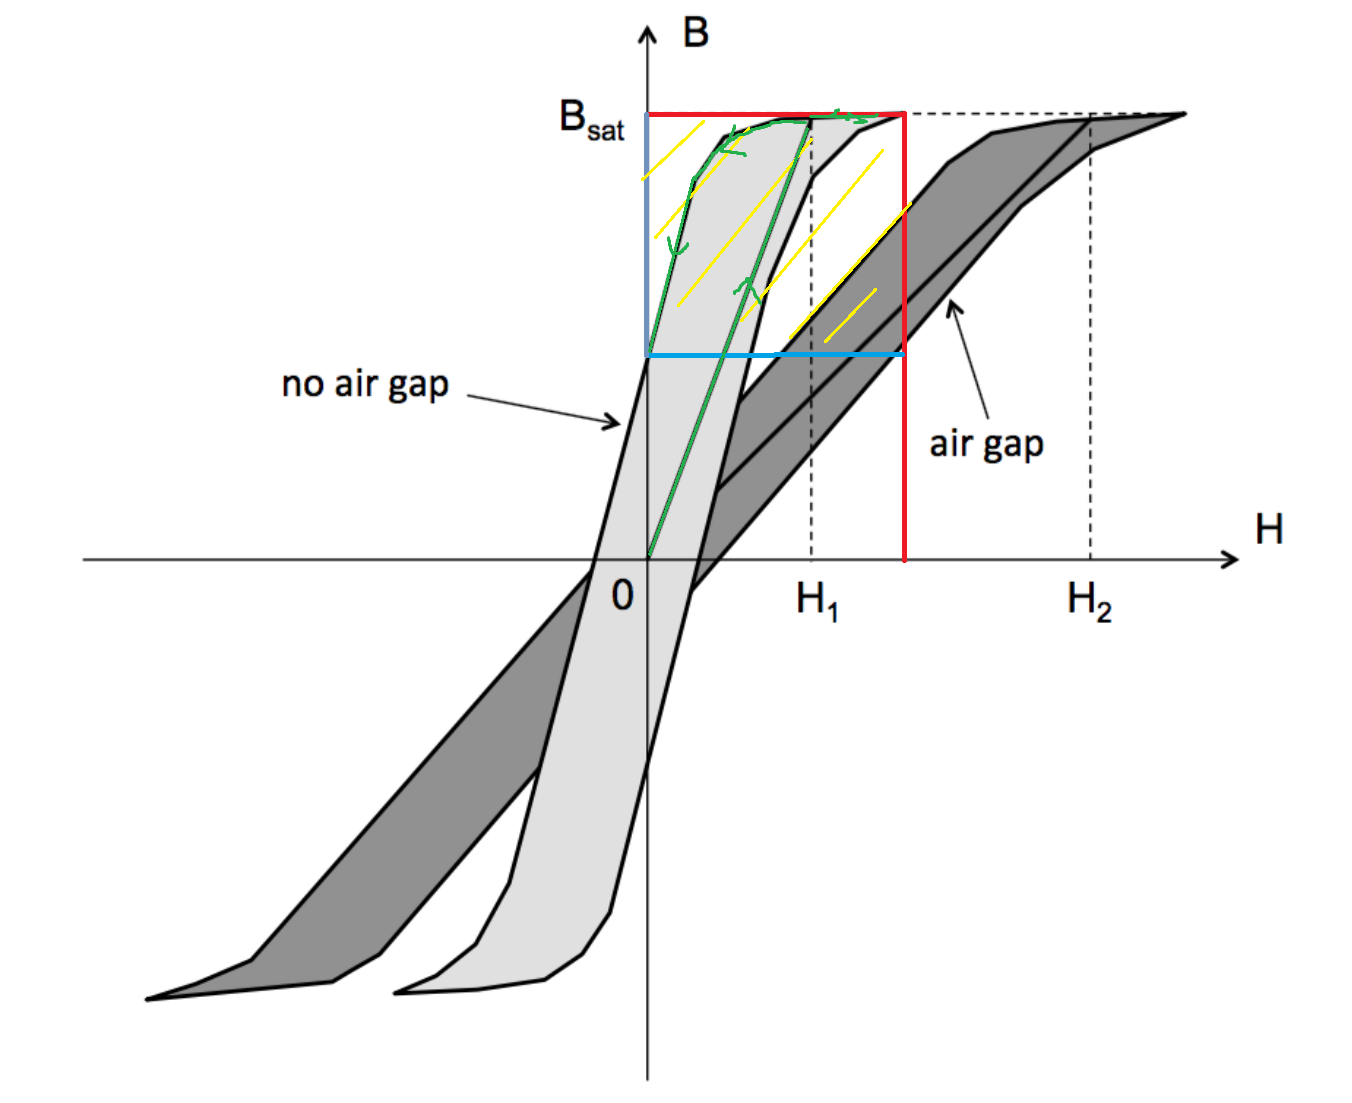
\includegraphics[width=0.5\textwidth]{../plots/electro_2_8.png}
\end{figure}

There is only partial recovery of the energy supplied to the inductor as the material is now magnetised. The magnetic field present in the core possesses energy that is not released when magnetisation is removed.

\subproblem{d}
Iron has a high susceptibility to boost the strength of the magnetic field in the core. It also has a high saturation field so that it can sustain a stronger field.

When used for alternating currents, however, the rapidly changing magnetic flux creates a large eddy current in the core due to the high conductivity of iron. This causes the core to heat up, a process that not only wastes energy but also may damage the core. This issue can be remedied by using laminated iron sheets instead of a solid iron core.
\qed


\end{document}